\section*{Problema 2}

\textbf{Implementa el algoritmo de Newton para calcular las raices del polinomio de Legendre $P_n(x)$}

\begin{equation*}
    x_{i+1} = x_i - \frac{P_n(x_i)}{P'_n(x_i)}
\end{equation*}

\textbf{Usando como puntos iniciales}

\begin{equation*}
    x_0 = cos \left (\frac{\pi(k+0.75)}{n+0.5}\right ) \qquad k=0,1,2,\dots,n
\end{equation*}

Se calcularon las raices para los polinomios de Legendre de grados $n=\{2,3,4,5,6,7\}$. Estos resultados se muestran en las tablas \ref{table:problema2_2}, \ref{table:problema2_3}, \ref{table:problema2_4}, \ref{table:problema2_5}, \ref{table:problema2_6} y \ref{table:problema2_7}. En la figura \ref{fig:problema2} se muestran los polinomios de Legendre en conjunto a sus raices.

\begin{table}[H]
    \centering
    \begin{tabular}{ccc} \hline
        \textbf{Punto} & $\mathbf{x_0}$ & \textbf{Raiz} \\ \hline
        0              & 0.587785       & 0.577350      \\
        1              & -0.587785      & -0.577350     \\ \hline
    \end{tabular}
    \caption{Raices del polinomio de Legendre de grado 2.}
    \label{table:problema2_2}
\end{table}

\begin{table}[H]
    \centering
    \begin{tabular}{ccc} \hline
        \textbf{Punto} & $\mathbf{x_0}$ & \textbf{Raiz} \\ \hline
        0              & 0.781831       & 0.774597      \\
        1              & 0.000000       & 0.000000      \\
        2              & -0.781831      & -0.781831     \\  \hline
    \end{tabular}
    \caption{Raices del polinomio de Legendre de grado 3.}
    \label{table:problema2_3}
\end{table}

\begin{table}[H]
    \centering
    \begin{tabular}{ccc} \hline
        \textbf{Punto} & $\mathbf{x_0}$ & \textbf{Raiz} \\ \hline
        0              & 0.866025       & 0.861136      \\
        1              & 0.342020       & 0.342020      \\
        2              & -0.342020      & -0.342020     \\
        3              & -0.866025      & -0.861136     \\ \hline
    \end{tabular}
    \caption{Raices del polinomio de Legendre de grado 4.}
    \label{table:problema2_4}
\end{table}

\begin{table}[H]
    \centering
    \begin{tabular}{ccc} \hline
        \textbf{Punto} & $\mathbf{x_0}$ & \textbf{Raiz} \\ \hline
        0              & 0.909632       & 0.906180      \\
        1              & 0.540641       & 0.540641      \\
        2              & 0.000000       & 0.000000      \\
        3              & -0.540641      & -0.538469     \\
        4              & -0.909632      & -0.909632     \\  \hline
    \end{tabular}
    \caption{Raices del polinomio de Legendre de grado 5.}
    \label{table:problema2_5}
\end{table}

\begin{table}[H]
    \centering
    \begin{tabular}{ccc}\hline
        \textbf{Punto} & $\mathbf{x_0}$ & \textbf{Raiz} \\ \hline
        0              & 0.935016       & 0.932470      \\
        1              & 0.663123       & 0.663123      \\
        2              & 0.239316       & 0.238619      \\
        3              & -0.239316      & -0.238619     \\
        4              & -0.663123      & -0.663123     \\
        5              & -0.935016      & -0.932470     \\ \hline
    \end{tabular}
    \caption{Raices del polinomio de Legendre de grado 6.}
    \label{table:problema2_6}
\end{table}

\begin{table}[H]
    \centering
    \begin{tabular}{ccc} \hline
        \textbf{Punto} & $\mathbf{x_0}$ & \textbf{Raiz} \\ \hline
        0              & 0.951057       & 0.949108      \\
        1              & 0.743145       & 0.743145      \\
        2              & 0.406737       & 0.405846      \\
        3              & 0.000000       & 0.000000      \\
        4              & -0.406737      & -0.406737     \\
        5              & -0.743145      & -0.741531     \\
        6              & -0.951057      & -0.951057     \\  \hline
    \end{tabular}
    \caption{Raices del polinomio de Legendre de grado 7.}
    \label{table:problema2_7}
\end{table}

\begin{figure}[H]
    \centering
    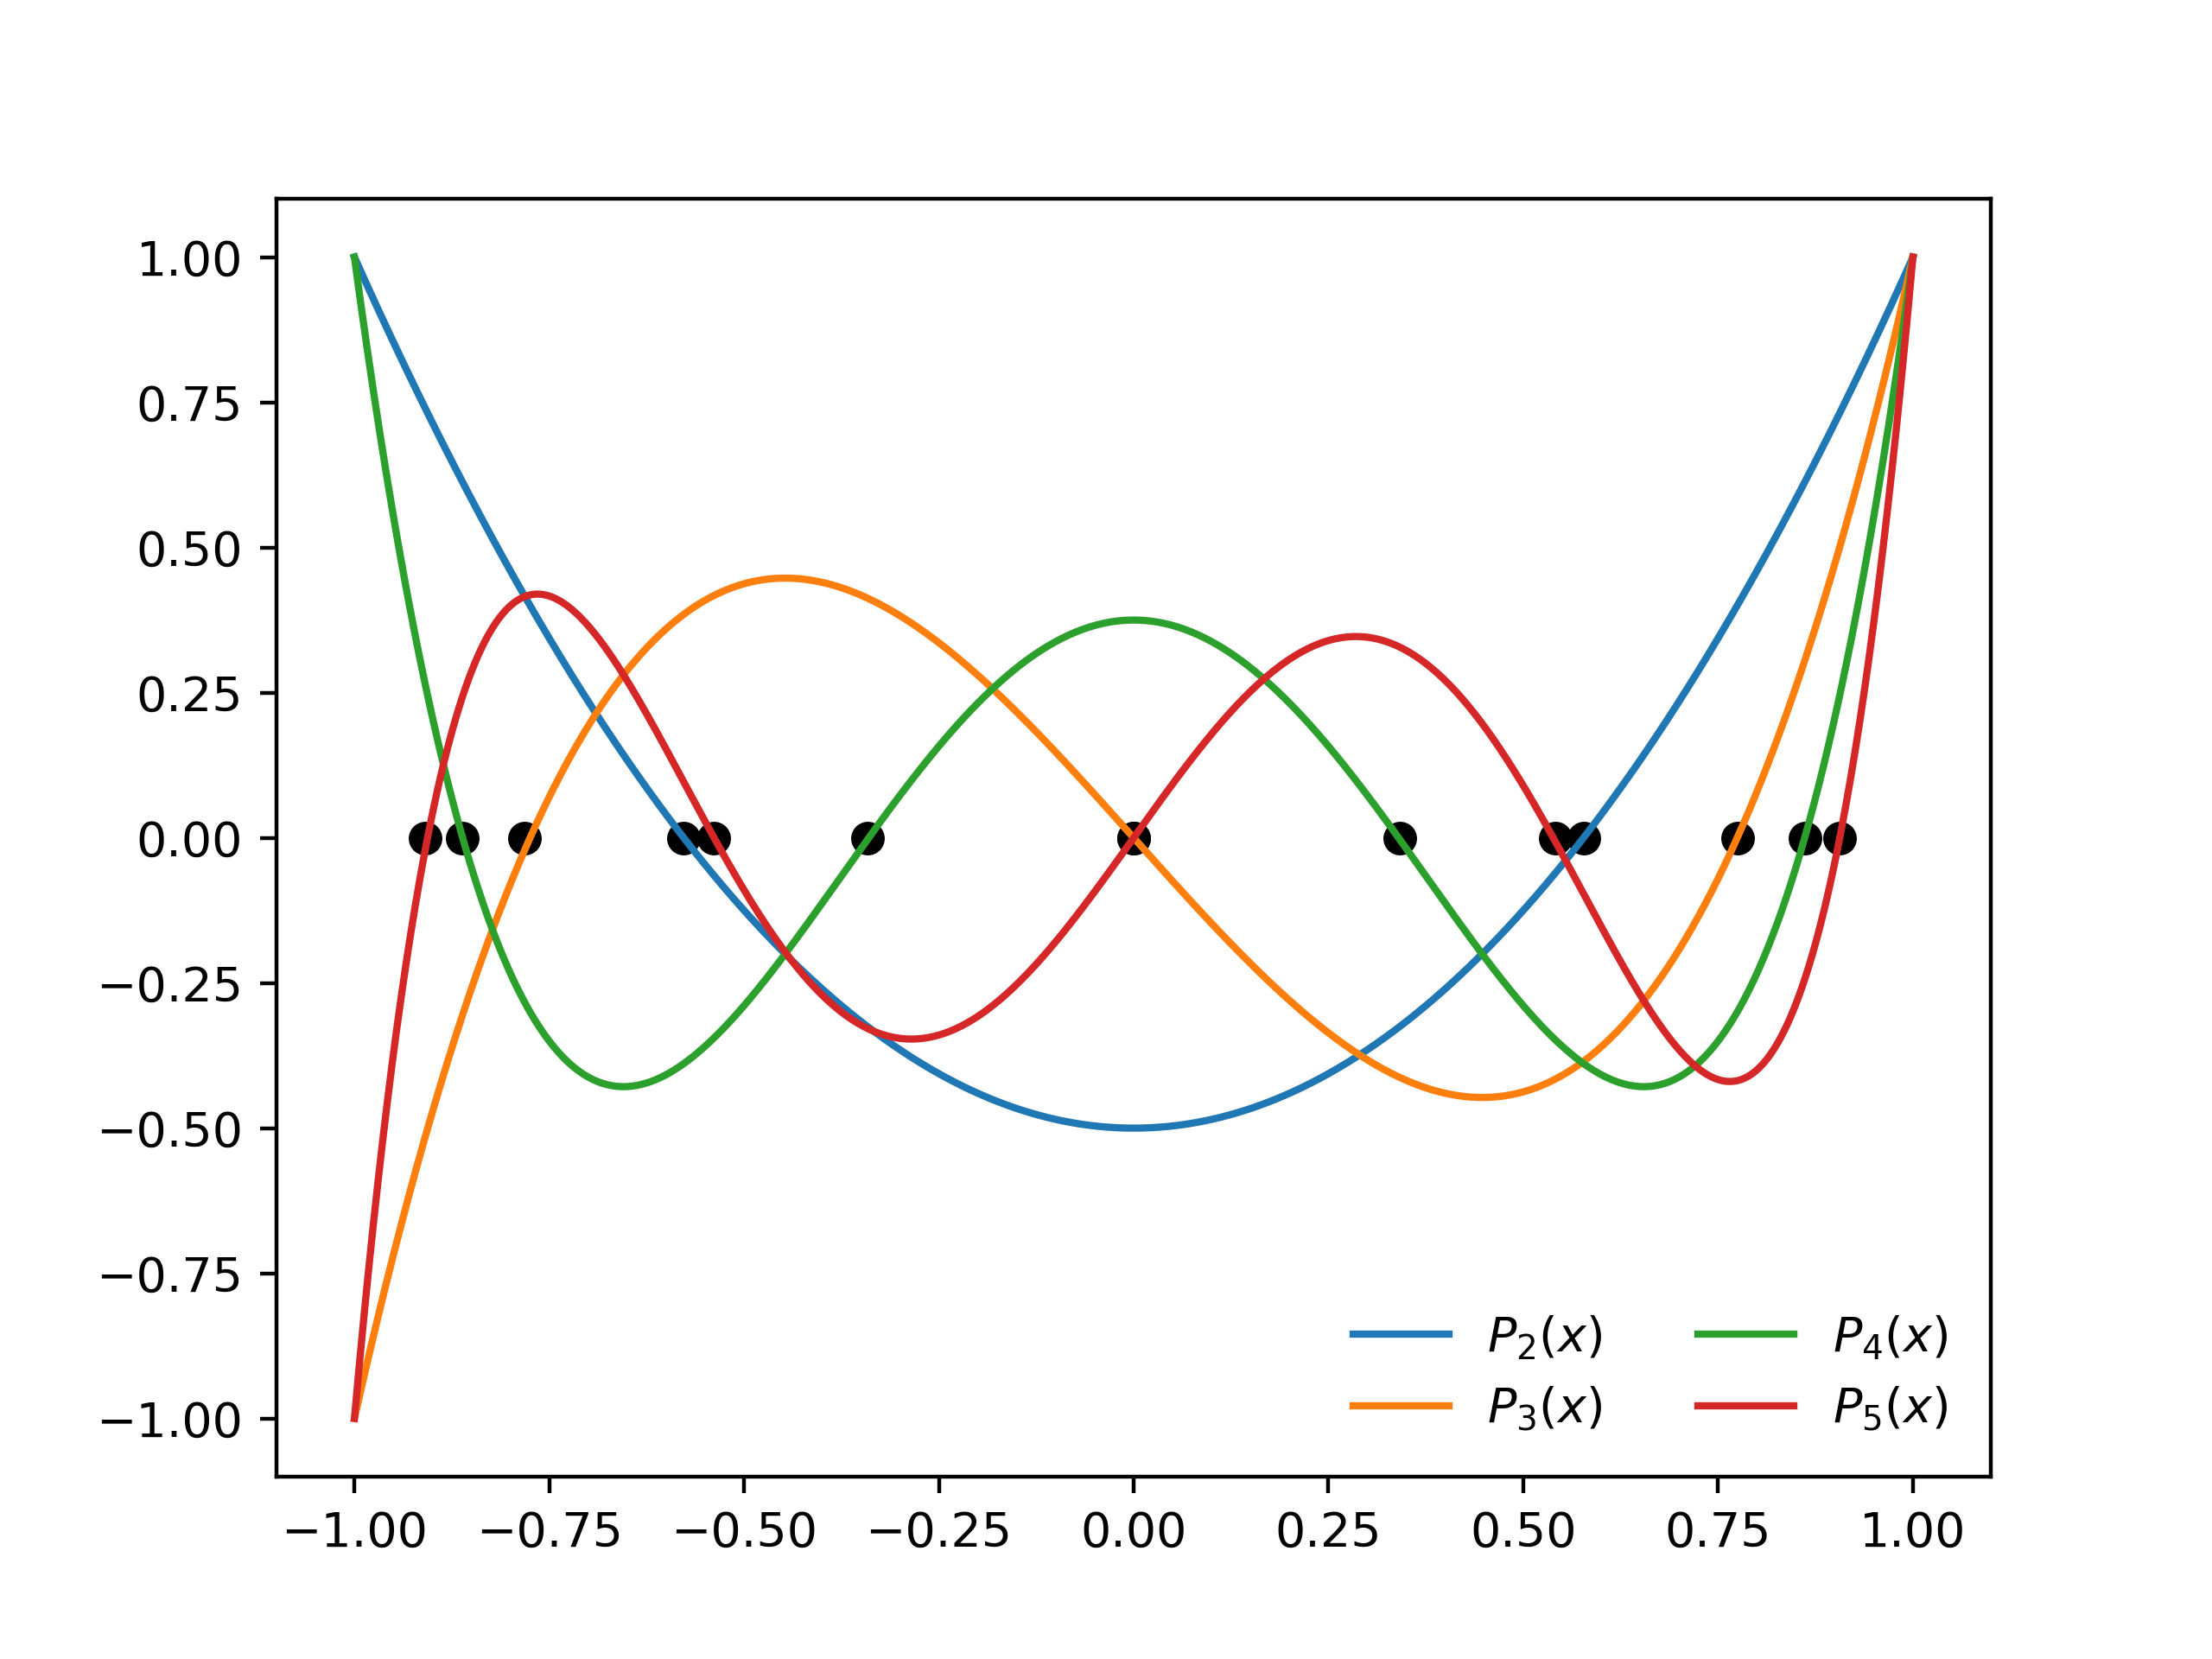
\includegraphics[width=16cm]{Graphics/problema2.png}
    \caption{Polinomios de Legendre de grado 2 al 7 en conjunto a sus raices.}
    \label{fig:problema2}
\end{figure}